\documentclass[11pt]{article}
\usepackage[a4paper, portrait, margin=1in]{geometry}
\usepackage{hyperref}
\usepackage{graphicx}
\usepackage{textcomp}
\usepackage{breakurl}
\usepackage{tabularx}
% Fancy header package for version number

\usepackage{fancyhdr}
\pagestyle{fancy}
\fancyhf{}
\renewcommand{\headrulewidth}{0pt}
\renewcommand{\footrulewidth}{0pt}

\fancypagestyle{firstpagefooter}
{
\lfoot{Version: 29.09.2016}
\cfoot{}
\rfoot{\thepage}
}
\cfoot{\thepage}

\begin{document}

\title{Advanced Systems Lab (Fall'16) -- First
Milestone}

\author{\textbf{Name: \emph{Aleksander Matusiak}}\\\textbf{Legi number: \emph{16-931-925}}}

\date{
\vspace{4cm}
\textbf{Grading} \\
\begin{tabular}{|c|c|}
\hline  \textbf{Section} & \textbf{Points} \\
\hline  1.1 &  \\ 
\hline  1.2 &  \\ 
\hline  1.3 &  \\ 
\hline  1.4 &  \\ 
\hline  2.1 &  \\ 
\hline  2.2 &  \\ 
\hline  3.1 &  \\ 
\hline  3.2 &  \\ 
\hline  3.3 &  \\ 
\hline \hline Total & \\
\hline 
\end{tabular} 
}

\maketitle
\thispagestyle{firstpagefooter}
\newpage

\section{System Description}\label{sec:system-description}

\subsection{Overall Architecture}\label{sec:desc:architecture}

The following figure\footnote{\url{https://gitlab.inf.ethz.ch/matusiaa/asl-fall16-project/blob/master/reports/milestone1/architecture.png}} includes provided system architecture with annotated instrumentation times names and names of classes that I have used in my implementation.
\smallskip

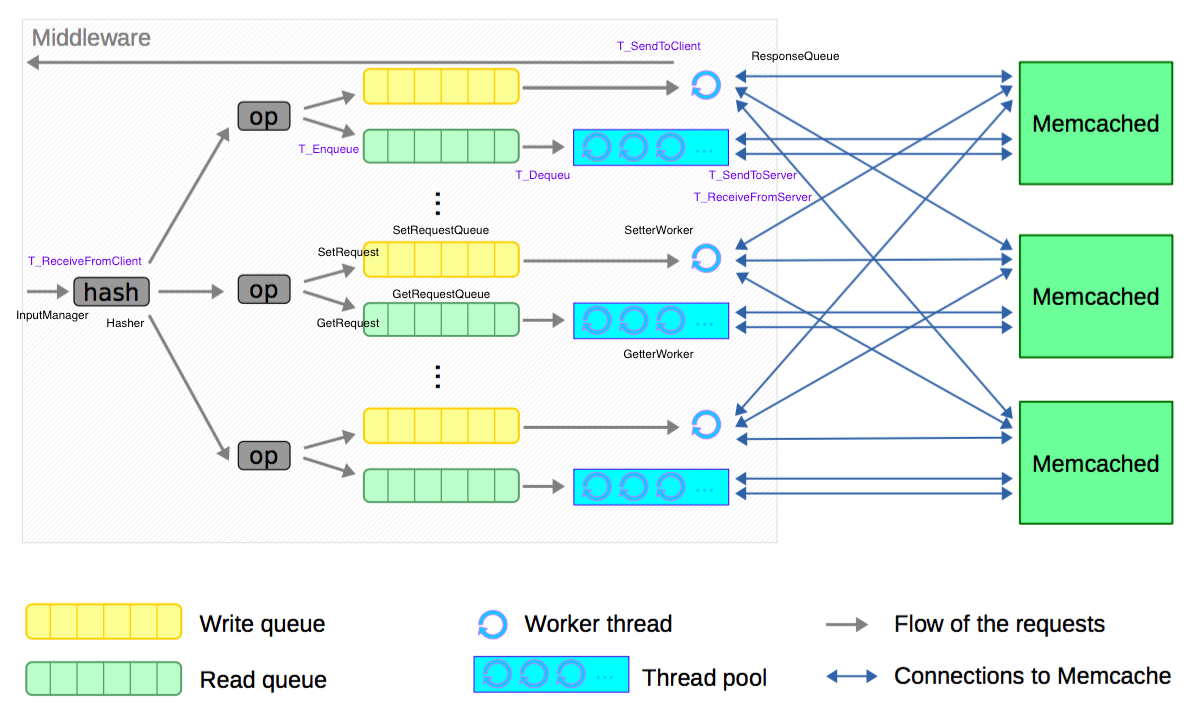
\includegraphics[scale=0.35]{architecture.png}
\smallskip

On the following class diagram\footnote{\url{https://gitlab.inf.ethz.ch/matusiaa/asl-fall16-project/blob/master/reports/milestone1/scheme.png}}  I have put most dependencies between classes, as well as important fields and methods. I have not included all of them, since some of them are not relevant to overall architecture. Some classes are implemented in a generic way, so class scheme represents only overall inheritance relationship, without mentioning exact generic types (for this, see the implementation).
\smallskip

\includegraphics[scale=0.33]{scheme.png}
\smallskip

The classes I created in my implementation are used for following purposes:
\begin{itemize}
\item MiddlewareServer\footnote{\url{https://gitlab.inf.ethz.ch/matusiaa/asl-fall16-project/blob/master/src/pl/matal/MiddlewareServer.java}} - main class responsible for linking all other objects and starting auxiliary threads.
\item InputManager\footnote{\url{https://gitlab.inf.ethz.ch/matusiaa/asl-fall16-project/blob/master/src/pl/matal/InputManager.java}} - class responsible to listening for incoming client connections and requests. It uses Java NIO selector. After it registers a request, it creates a Request object and passes it to MiddlewareServer. The InputManager counts the number of get and set requests and designates requests that should be logged later.
\item Hasher\footnote{\url{https://gitlab.inf.ethz.ch/matusiaa/asl-fall16-project/blob/master/src/pl/matal/Hasher.java}} - responsible for assigning server number to the  given request based on its key. See \ref{sec:desc:hashing}.
\item MemcachedServer\footnote{\url{https://gitlab.inf.ethz.ch/matusiaa/asl-fall16-project/blob/master/src/pl/matal/MemcachedServer.java}} - class representing memcached servers, which keeps host and port of this server. It also initializes the connection to the servers (Java NIO or normal Java socket) and returns an appropriate socket object.

\item Request\footnote{\url{https://gitlab.inf.ethz.ch/matusiaa/asl-fall16-project/blob/master/src/pl/matal/Request.java}} - abstract class representing incoming client request. It has 2 subclasses: GetRequest\footnote{\url{https://gitlab.inf.ethz.ch/matusiaa/asl-fall16-project/blob/master/src/pl/matal/GetRequest.java}} and SetRequest\footnote{\url{https://gitlab.inf.ethz.ch/matusiaa/asl-fall16-project/blob/master/src/pl/matal/SetRequest.java}}, corresponding to appropriate type of requests (SetRequest is also used for representing delete requests). Each Request has an associated SocketChannel to which worker thread should write its response. For each request we also remember instrumentation times and flags: whether the request was successful and whether we should log it. SetRequest class consists additionally of params table and value to be stored.

\item RequestQueue\footnote{\url{https://gitlab.inf.ethz.ch/matusiaa/asl-fall16-project/blob/master/src/pl/matal/RequestQueue.java}} - abstract class representing queue in which requests are stored. Class is parametrized by type R, which corresponds to stored requests class (so either GetRequest or SetRequest). It consists of blocking queue and exposes methods for adding requests to the queue, as well as getting elements from the queue in a blocking (used by GetWorkers) or non-blocking (used for SetWorkers) way. This class has 2 subclasses: GetRequestQueue\footnote{\url{https://gitlab.inf.ethz.ch/matusiaa/asl-fall16-project/blob/master/src/pl/matal/GetRequestQueue.java}} and SetRequestQueue\footnote{\url{https://gitlab.inf.ethz.ch/matusiaa/asl-fall16-project/blob/master/src/pl/matal/SetRequestQueue.java}} (extending RequestQueue$<$GetRequest$>$ and RequestQueue$<$SetRequest$>$), which additionally store a single one (GetRequestQueue) or a list (SetRequestQueue) of MemcachedServer objects.
\item Worker\footnote{\url{https://gitlab.inf.ethz.ch/matusiaa/asl-fall16-project/blob/master/src/pl/matal/Worker.java}} - abstract class responsible for processing elements from an appropriate queue, sending requests to memcached servers and sending response to the client. It implements Runnable interface, so that for each worker we can create a separate thread. It is also parametrized by queue and request types. It has 2 subclasses GetterWorker\footnote{\url{https://gitlab.inf.ethz.ch/matusiaa/asl-fall16-project/blob/master/src/pl/matal/GetterWorker.java}} and SetterWorker\footnote{\url{https://gitlab.inf.ethz.ch/matusiaa/asl-fall16-project/blob/master/src/pl/matal/SetterWorker.java}} which handle appropriate requests from appropriate queues.
\item ResponseQueue\footnote{\url{https://gitlab.inf.ethz.ch/matusiaa/asl-fall16-project/blob/master/src/pl/matal/ResponseQueue.java}} and ResponseQueueNode\footnote{\url{https://gitlab.inf.ethz.ch/matusiaa/asl-fall16-project/blob/master/src/pl/matal/ResponseQueueNode.java}} - responsible for storing responses for set requests to multiple servers. See \ref{sec:desc:writes}. 

\end{itemize} 

\subsection{Load Balancing and Hashing}\label{sec:desc:hashing}

For hashing I have used a function similar to this implemented in Java to get hash values of strings. Let $a_na_{n-1}...a_2a_1$ be the key to be hashed, $a_n$, $a_{n-1}$, ... $a_2$, $a_1$ consecutive letters (bytes) starting from the first one from the left. Then we define hash function as follows:
$$h(a_na_{n-1}...a_2a_1) = B^{n-1}a_n + B^{n-2}a_{n-1} + ... Ba_2 + a_1,$$
where for $B$ I have chosen 257, which is a prime number and is bigger than possible value of byte. The value of the hash can be easily computed using Horner's scheme. These operations are being done using Java {\it int} type, so if during execution the value exceeds maximum value of {\it int}, it overflows and goes to the minimum value. This, however, is not a problem, since we are not trying to avoid conflicts (then we would use {\it long} type) and either way we have to assign a server number from a small range. 

To calculate a server number based on the hash value, I have used consistent hashing presented during a tutorial session. If $n$ is the number of servers, we divide the interval: \begin{verbatim} (Integer.MIN_VALUE, Integer.MAX_VALUE)\end{verbatim} to $n$ intervals of equal length and assign a server depending to which interval does the hash value belong.

Algorithm described above for calculating a hash function is commonly used while implementing text algorithms which use hashing. It is known to be effective and create a low amount of conflicts. This also means, that it uniformly distributes the values of the function. What is more, the value of the hash function is dependent on each character of the key, so changing one of them would change the result value (more or less significantly depending on the position of the character). Using consistent hashing presented during a tutorial session enables us then to get a uniform distribution of keys to servers. To prove this, I have measured the distribution of server load during my stability experiment and have achieved following results:

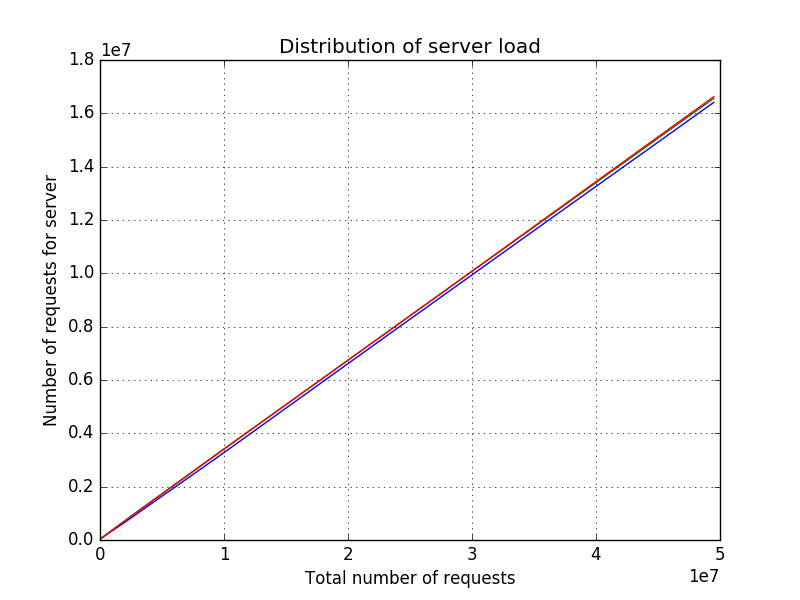
\includegraphics[scale=0.6]{servers_distribution.png}

Each line on the plot corresponds to load of one server. As we can see, during the stability experiment (one hour), each server had similar overall load to other ones. At the end of the experiment I have achieved the following overall loads:
\medskip

\begin{tabular}{|c|c|c|c|c|}
\hline &  \textbf{Total} & \textbf{Server 1} & \textbf{Server 2} & \textbf{Server 3} \\
\hline Number of requests & 49600000 & 16412642 & 16561949 & 16625409 \\
\hline
\end{tabular} 
\medskip

This means, that maximum deviation from the average was only $7,3$\textperthousand, which can be considered as satisfactory load balancing factor.

\subsection{Write Operations and Replication}\label{sec:desc:writes}

According to the initial specification, we were only allowed to use one thread for write worker. However, this worker has to listen to two events: new objects in the queue and responses from the server. None of this operation could be blocking, since it would block or severely damage the performance of the worker. This is why I had to use active waiting as a way to provide satisfactory performance of setter worker. More precisely, each worker thread which sends ``set" requests (later called {\it setter worker} or {\it setter thread}) runs an infinite loop. In this loop it firstly checks if there is any response from server waiting (using non-blocking operations on a selector) and if yes, it handles it. Later in the loop it checks, also in a non-blocking manner, whether there is a new request in the queue. If yes, it handles it. This loop will be later referred to as {\it main loop}. The active waiting is a very bad design pattern, since the processor core spends all its resources on executing this loop. However, we will use the system under heavy workload so using that many resources should not be an issue here (the usage of resources will correspond to the load of the system).

Since write workers send requests to several servers and do not wait for the response, it was necessary to introduce a mechanism for collecting responses from the server. I have used an own data structure based on LinkedList and implemented by ResponseQueue class. Each node in the list (represented by ResponseQueueNode object) corresponds to a request sent to multiple servers. For each server we keep pointers to the node with the request to which response should come first from this server. When the structure is notified that the new request is to be sent to the servers, it adds a new node corresponding to this request at the end of the list. When we receive response from the server we can move its pointer to the next node. The correctness of this method is based on the fact that TCP protocol guarantees that the responses from one server will be in the same order as sent requests.

We have to remember, that requests to some servers can result in error and we have to send an aggregated response. This is why each ResponseNode object contains also a success flag and an optional error message. If we get an error from one of the servers, then we will send this error later to the client.

Once all the pointers are behind first node of the list, we send an aggregated response for the corresponding request and remove it from the list. If the request is supposed to be logged, we log it. It is worth noticing that for sending a response (both for ``set" and ``get" requests) we use the Socket object from which we got a request from the client and which has been stored with the request. 

In the ``write one`` scenario it would not be necessary to use such a structure. Simple queue would be enough - once we send request we add the request at the end, once we get a response - we take a corresponding request from the beginning.

The latencies that the writing operation will incur will have main source in network latencies. Using middleware requires additional network connections, which is a huge overhead and it will probably limit the throughput for set (and get) requests. Additional latencies may be introduced by the time the request spend in the queue. This might be significant if the percentage of set requests is high and we replicate requests to several servers. Then worker thread would have to handle sending several messages and receiving response, which may cause queue to grow longer and worker thread not being able to instantly forward the request. Collecting responses using a queue can also increase the response time, since we have to parse every response and check whether it was successful or not. Logging requests is also connected with additional overhead, since we have to write logs on standard output and into the log file.  

If we assume that time spent by the request in the network is most significant one, then the replicated case should not incur that much latencies, since we send requests asynchronously. However, since we have to wait for many responses, if one of them is taking longer to be passed in the network and processed by the server then the overall time for the request would also increase. Therefore, the additional latencies may be connected with instability of the network.

\subsection{Read Operations and Thread Pool}\label{sec:desc:reads}

We create the threads responsible for handling ``get" requests (later called {\it getter workers} or {\it getter threads}) during the creation of the server. When we start the server, we start each of the thread. Each getter worker initiates a connection with the memcached server assigned to the given queue shortly after the program has started. Each connection is represented by a Java Socket object. This connection is later kept open all the time and all requests from the thread are sent using this connection. This solutions enables us to minimize network overhead, because we don't need to initiate a TCP connection every time we want to send a request, which could take some time (three-way handshake would create additional overhead). What is more, main use case of memcached according to the documentation is having many requests from a client to which we are constantly connected.

Threads can access ``get" requests from the queue implemented by the GetRequestQueue class. As an underlying data structure I have used BlockingQueue. This structure is thread safe and enables each getter worker to wait for a new element, if the queue is empty at the moment. Once new element is added to the queue, one of the waiting thread can access it, remove it from the queue and process it.

When the thread takes a request out of the queue, it constructs an appropriate String (and later ByteBuffer[]) object containing a request and sends it to the memcached server using previously created Socket object. Once the thread sends a request, it waits for the response. This is a blocking operation and the thread does not perform any other actions in the meantime. When the thread receives response from the server it checks, whether the response has been successful and forwards the response to the client. If the request is supposed to be logged, the getter thread does that.

\section{Memcached Baselines}\label{sec:baseline}

This experiments were conducted using the following provided scheme:
\medskip

\small{
\smallskip
\begin{tabular}{|c|c|}
\hline Number of servers & 1 \\ 
\hline Number of client machines & 2 \\ 
\hline Virtual clients / machine & 1 to 64 \\ 
\hline Workload & Key 16B, Value 128B, Writes 1\% \\
\hline Middleware & Not present \\ 
\hline Runtime x repetitions & 30s x 5 \\ 
\hline Log files & logs\_baseline\_1, logs\_baseline\_2, logs\_baseline\_cumulative \\
\hline 
\end{tabular} }
\medskip

During every experiment (both for baseline and stability) we use the following units:
\begin{itemize}
\item throughput - operations per second,
\item response time - in microseconds,
\item time (current duration of the experiments) - in seconds.
\end{itemize}
Each log file which is not log from memaslap, starts with the line describing the content of the columns.

The number of clients for each experiment has been increased by one on each of the client machines, which means that the total number of client was always odd. This enabled us to have the same load on both client machines so that the results would not by influenced by different performance of each client machine under different load. 

\subsection{Throughput}\label{sec:baseline:tput}
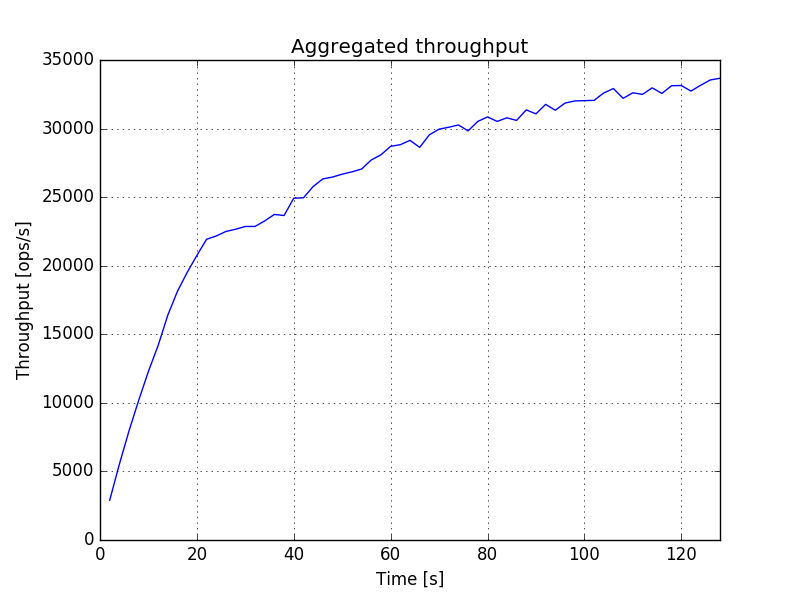
\includegraphics[scale=0.7]{baseline_throughput.png}
\medskip

Till 24 clients the throughput is increasing significantly. This is is understandable since for small number of clients server is underloaded and can handle requests from new clients very effectively. With more clients throughput still increases, but a little bit slower, till around 96 clients. Then throughput increases even slower. We can therefore conclude that since 96 clients server becomes saturated. We can see that throughput is constantly increasing as you increase number of clients, so we can say that memcached server has not encountered problems connected with too high number of clients.

\subsection{Response time}\label{sec:baseline:rt}

In the following figure $y$-axis has been limited to start from 0. Even though standard deviation markers can go below 0, it does not give us any information. The same approach will be used in stability response time plot.

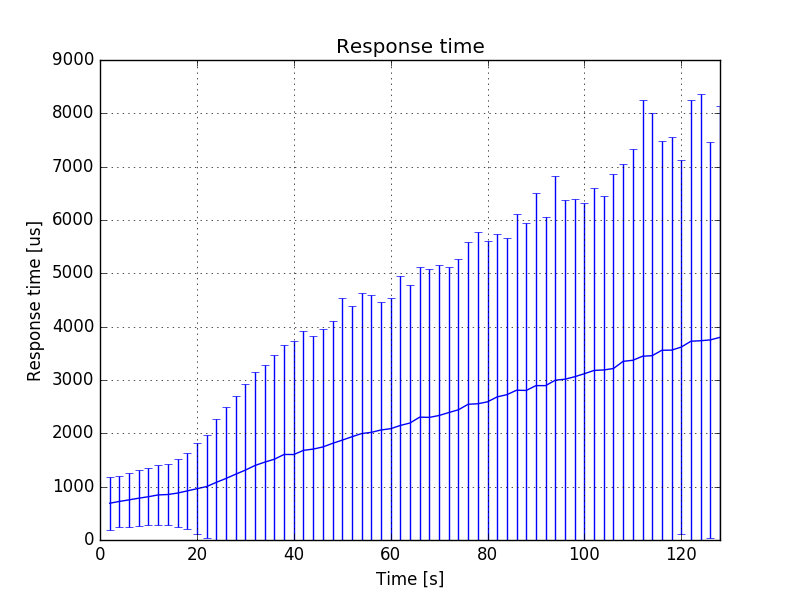
\includegraphics[scale=0.7]{baseline_response_time.png}
\medskip

From above plot we can see, that average response time changes almost in a linear way as we increase the number of clients. The performance of memcached server is therefore pretty predictable. Since memcached uses only one thread, we do not see the period where response time is almost constant - all requests have to be queued, from which follows that more clients means higher response time.

We can see that response times increases slightly more dynamic since around 24 clients, which is consistent with the behavior of throughput at that point. However, at 96 clients we cannot see a drastic increase in the average response time, so based on this plot we can say that server has not been saturated yet. We do not find any drastic increase in the average response time, so we can once again say, that server has not encountered problems connected with too high number of clients.

However, the standard deviation for every measurement is really high. This is the result of the fact that clients and server work on different machines and they have to communicate through network. Depending on the current load of network, times that it takes from packet to reach server and return back to client can differ significantly.

\section{Stability Trace}\label{sec:trace}

This experiment was conducted using the following provided scheme:
\medskip

\small{
\smallskip
\begin{tabular}{|c|c|}
\hline Number of servers & 3 \\ 
\hline Number of client machines & 3 \\ 
\hline Virtual clients / machine &  64 \\ 
\hline Workload & Key 16B, Value 128B, Writes 1\% \\
\hline Middleware & Replicate to all (R=3) \\ 
\hline Runtime x repetitions & 1h x 1 \\ 
\hline Log files & logs\_stability\_1, logs\_stability\_2, logs\_stability\_3, stability\_parsed \\
\hline 
\end{tabular} }
\medskip

The number of threads in a thread pool for each getter thread was 16. Values have been measured every 10 seconds.

\subsection{Throughput}
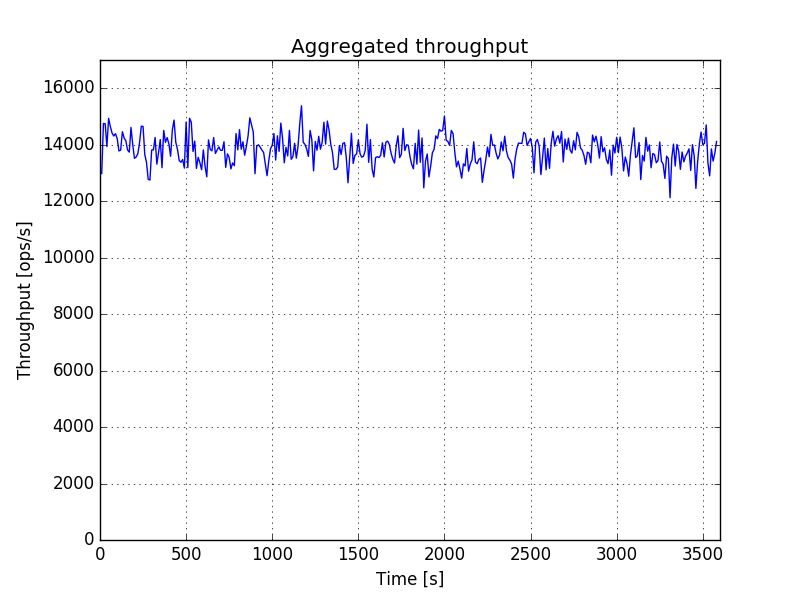
\includegraphics[scale=0.7]{stability_throughput.png}

Above figure shows us that the middleware was performing in a considerably stable way when it comes to throughput. Spikes visible on the plot are understandable since requests go over network, which introduce additional instability.

\subsection{Response time}

On below plot standard deviation has been marked by additional series (red and green) - using standard solution with vertical lines would drastically decrease the clarity of the plot due to big density of the points.

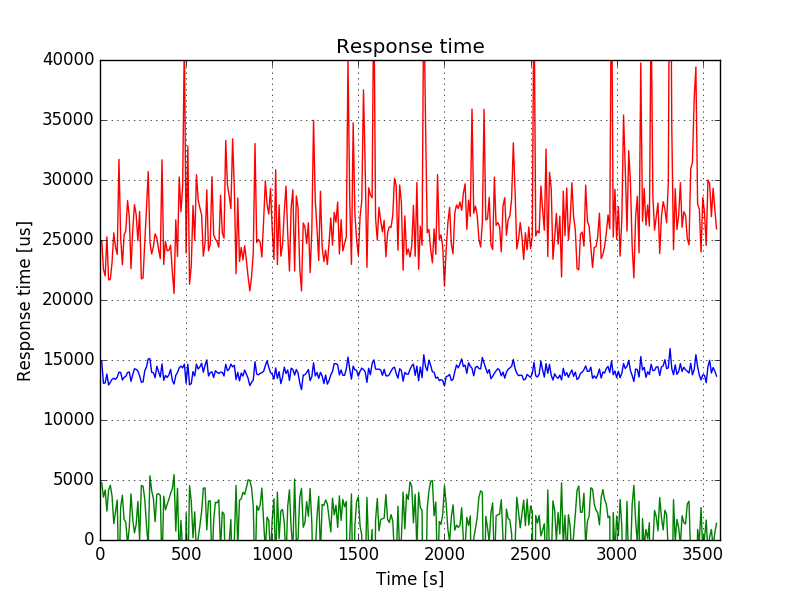
\includegraphics[scale=0.7]{stability_response_time.png}

The average response time is also pretty stable, but we can see pretty big standard deviation of the measurements of response time. However, baseline experiments also had big standard deviations, from which we can conclude that the middleware is not to blame for it, but the underlying cause lays in the network latency and instability.

\subsection{Overhead of middleware}

In the baseline experiments for 64 clients load for one server equals 64 clients. Since the hashing we used is uniform and set requests (and replication they are connected with) stand for only 1\%, for stability experiment with 192 clients and 3 servers we also have load 64 clients per server.  This is why we will compare the results of the stability experiment with the results of baseline experiment with 64 clients. We would have to then calculate an average throughput for one server.

In the below table we compare the aggregated throughput and average response time for baseline and stability experiment (rounded to integers). The overhead column stands for middleware value divided by baseline value.
\medskip

\begin{tabular}{|c|c|c|c|}
\hline & \textbf{Baseline}& \textbf{Middleware} & \textbf{Overhead} \\ 
\hline Clients & 64 & 192 & - \\
\hline Memcached servers & 1 & 3 & - \\
\hline Load per server [clients] & 64 & 64 & -\\
\hline Aggregated throughput [ops/s] & 29143 & 14289 & - \\ 
\hline Throughput per server [ops/s] & 29143 & 4763 ($= 14289/3$) & 0.163 \\
\hline Response time [us] & 2193 & 13491 & 6.15 \\
\hline Response time standard deviation & 2589 & 10888 & - \\
\hline Coefficient of variation & 1.18 & 0.81 & 0.68 \\
\hline 
\end{tabular}
\medskip

As we can see from the table, introducing middleware was connected with additional overhead for throughput and response time. The response time has increased around 6 times, while throughput has decreased around 6 times. This can be caused by several factors. 

The number of network connections with introduced middleware is bigger - we have to connect both client to middleware and middleware to the server. This introduces additional overhead, because we have to send network messages more often. Since we don't know the topology of the network in which clients and servers run, the distances between hosts can be big and additional connections only increase the total distance that a request hast to travel. 

What is more, during the middleware experiments the load of the network is increased which may cause higher network latencies. This is because we have more clients and servers than in the corresponding baseline experiments and we replicate every set request to additional two servers.

Replication can also cause an increase in the response time. In the middleware experiment we replicate every set request to three servers, which takes some time and increases waiting time, because with 3 messages we are more prone to network latencies.

We can also say that the mecached load changes. Since it has only one thread, it has to queue additional coming requests. However, it's difficult to estimate how much it changes, since we haven't analyzed yet the instrumentation time. I would not consider it a very important factor when it comes to overhead.

What is more, the number of threads in thread pools was chosen not based on experiments, but rather on personal assumptions, therefore it might not be optimal.

It is also worth noticing that standard deviation for response time has improved by introducing middleware. This might be because requests now spend more time being processed by the middleware and are less prone to network latencies and instability.

\pagebreak

\section*{Logfile listing}

\begin{tabular}{|c|p{12.0cm}|}
\hline \textbf{Short name }& \textbf{Location} \\ 
\hline logs\_baseline\_1 & \url{https://gitlab.inf.ethz.ch/matusiaa/asl-fall16-project/blob/master/logs/milestone1/logs_baseline_1.tar.gz}\\ 
\hline logs\_baseline\_2 & \url{https://gitlab.inf.ethz.ch/matusiaa/asl-fall16-project/blob/master/logs/milestone1/logs_baseline_2.tar.gz}\\ 
\hline logs\_baseline\_cumulative & \url{https://gitlab.inf.ethz.ch/matusiaa/asl-fall16-project/blob/master/logs/milestone1/logs_baseline_cumulative.tar.gz}\\ 
\hline logs\_stability\_1 & \url{https://gitlab.inf.ethz.ch/matusiaa/asl-fall16-project/blob/master/logs/milestone1/logs_stability_1.tar.gz}\\ 
\hline logs\_stability\_2 & \url{https://gitlab.inf.ethz.ch/matusiaa/asl-fall16-project/blob/master/logs/milestone1/logs_stability_2.tar.gz}\\ 
\hline logs\_stability\_3 & \url{https://gitlab.inf.ethz.ch/matusiaa/asl-fall16-project/blob/master/logs/milestone1/logs_stability_3.tar.gz}\\ 
\hline stability\_parsed & \url{https://gitlab.inf.ethz.ch/matusiaa/asl-fall16-project/blob/master/logs/milestone1/stability_parsed.log}\\ 
\hline 
\end{tabular}

\end{document}
